%%%%%%%%%%%%%%%%%%%%%%%%%%%%%%%%%%%%%%%%%%%%%%%%%%%%%%%%%%%%%%%%%%%%%
%% This is a (brief) model paper using the achemso class
%% The document class accepts keyval options, which should include
%% the target journal and optionally the manuscript type. 
%%%%%%%%%%%%%%%%%%%%%%%%%%%%%%%%%%%%%%%%%%%%%%%%%%%%%%%%%%%%%%%%%%%%%
\documentclass[journal=jacsat]{achemso}
\setkeys{acs}{articletitle = true}
\usepackage{enumitem}
\usepackage{array}
\usepackage{epstopdf}
\usepackage{graphicx}
\newcolumntype{L}[1]{>{\raggedright\let\newline\\\arraybackslash\hspace{0pt}}m{#1}}
\newcolumntype{C}[1]{>{\centering\let\newline\\\arraybackslash\hspace{0pt}}m{#1}}
\newcolumntype{R}[1]{>{\raggedleft\let\newline\\\arraybackslash\hspace{0pt}}m{#1}}


%%%%%%%%%%%%%%%%%%%%%%%%%%%%%%%%%%%%%%%%%%%%%%%%%%%%%%%%%%%%%%%%%%%%%
%% Place any additional packages needed here.  Only include packages
%% which are essential, to avoid problems later. Do NOT use any
%% packages which require e-TeX (for example etoolbox): the e-TeX
%% extensions are not currently available on the ACS conversion
%% servers.
%%%%%%%%%%%%%%%%%%%%%%%%%%%%%%%%%%%%%%%%%%%%%%%%%%%%%%%%%%%%%%%%%%%%%
\usepackage[version=3]{mhchem} % Formula subscripts using \ce{}
\usepackage{epstopdf}
\usepackage{enumitem}
\newcommand*\mycommand[1]{\texttt{\emph{#1}}}
\author{Sridhar Neelamraju}
\email{sridharn@ncbs.res.in}
\affiliation[NCBS]{Simons Centre for the Study of Living Machines, National Centre for Biological Sciences, Tata Institute of Fundamental Research}
\alsoaffiliation[Cam]{University of Cambridge, University Chemical Laboratories, Lensfield Road, Cambridge CB2 1EW, U.K}
\author{Shachi Gosavi}
\affiliation[NCBS]{Simons Centre for the Study of Living Machines, National Centre for Biological Sciences, Tata Institute of Fundamental Research}
\email{shachi@ncbs.res.in}
\author{David J. Wales}
\email{dw34@cam.ac.uk}
\affiliation[Cam]{University of Cambridge, University Chemical Laboratories, Lensfield Road, Cambridge CB2 1EW, U.K}

%\phone{+123 (0)123 4445556}
%\fax{+123 (0)123 4445557}
\title[Roy]
  {Energy landscape of a 5$_2$ knotted protein from discrete path sampling}
%\abbreviations{IR,NMR,UV}
\keywords{Energy landscape, Go models, structure based models, protein folding, knotted proteins, Gordian knot, UCH-L1}

%%%%%%%%%
\begin{document}
%%%%%%%%%%%%%%%%%%%%%%%%%%%%%%%%%%%%%%%%%%%%%%%%%%%%%%%%%%%%%%%%%%%%%
\begin{abstract}
%In the abstract, go the other way. First talk about how calculating the energy landscape is useful for topologically complex proteins of which knots is an extreme case. Then say here using a knotted protein, UCH-L1, we provide a tutorial. A sentence about UCH-L1 and its knot and then what do you learn from the landscape.

It is remarkable that proteins can form knots with complex topologies with and without the aid of the cellular machinery. Knots are conserved across protein families indicating that knotting can be important for function. Computational, mathematical and experimental approaches have been used to investigate the mechanism of knot formation. Discrete Path Sampling, in combination with a coarse-grained potentials like Structure Based models provides a method to capture multiple distinct folding mechanisms that can exist as parallel pathways in knotted proteins. The pathways are extracted from a network of connected local minima and transition states visualised as a disconnectivity graph. From this network, we identify likely intermediate states, topological barriers to formation of a knot, and show how the different types of folding mechanisms can coexist for a protein with 231 residues that forms a 5$_2$ Gordian knot. With a step-by-step guide to using discrete path sampling,  we show that the method reproduces folding pathways obtained from molecular dynamics with a potential similar to ours. Additionally, we identify low-energy topolological traps and quantify the potential energy barriers which separate them from the native knotted state.  We show that discrete path sampling provides an efficient framework for sampling energy landscapes of proteins with complex entangled topologies. 
\end{abstract}


\section{Introduction}
The monomeric Ubiquitin C-terminal Hydrolase isoenzyme L1 (UCH-L1) is a deubiquitinating enzyme that cleaves ubiquitin at its carboxyl terminal.  It is highly expressed in neurons and accounts for 1–2\% of the brain proteome\cite{Wilkinson89}.  It is linked to neurodegenerative diseases such as Parkinson’s\cite{Marganore04a} and Alzheimer’s\cite{Zhangm14a}. Its presence and function as a deubiquitinating enzyme is also associated with tumours of the brain and the upper respiratory tract\cite{Ummanni11a,Goto15a,Norton86a,Liu03a,Liu09a}. UCH-L1 has six $\beta$-strands that form a $\beta$-sheet  surrounded by 10 $\alpha$-helices.  The 231 residues form a secondary structure that folds into a 5$_2$ or Gordian knot. Of these,  216 residues are part of a knotted core, 5 unstructured residues form the tail on the N-terminal and 10 residues form the tail on the C-terminal\cite{Zhao18a,Sulkowska20a}. 

The folding behaviour of UCH-L1 has been studied with both experimental\cite{Lou16a,Lee18a,Bishop16a,Das06a,Zhang16a,Andersson09a} and computational molecular dynamics methods\cite{Zhao18a}. With solution Nuclear Magnetic Resonance\cite{Lou16a,Lee18a}, it was noted that two distinct kinetic folding intermediates are transiently populated on two distinct parallel pathways between the unfolded and native states. Mechanical unfolding and refolding experiments with single-molecule force spectroscopy\cite{Ziegler16a} detected many on- and off-pathway intermediates. Finally, molecular dynamics simulations with a coarse-grained Structure-Based Model (SBM) at folding temperature identified two topologically distinct (un)folding pathways: One where the 5$_2$ knot unfolded via a 3$_1$ intermediate structure before unknotting, and another, where the 5$_2$ knot  directly unfolded to the unknotted structure.

Given the number and heterogeneity of intermediates observed, and the possibility of distinct parallel pathways involved in the unfolding of this complex protein, together with the fact that knotted proteins fold/unfold on timescales of minutes, constructing a detailed potential energy landscape of a 5$_2$ protein is a fascinating challenge. Here, we employ a combination of discrete path sampling\cite{DPS1}(DPS) and Structure-Based Models (SBMs)\cite{Neelamraju20a,Neelamraju19a,Neelamraju18a,smog} to describe the energy landscape of the UCH-L1 in great detail. From a database containing a few tens of thousands of local minima and transition states, we identify topological traps, potential energy barriers that separate the topological traps from the native state and multiple pathways that connect the unknotted/unfolded state to the native-knotted state. It is important to understand as many distinct folding pathways as possible, as some of these might be activated or deactivated within the crowded environs of a cell\cite{Aaden14a}, or while folding co-translationally\cite{Bitran20a}. Given the functional importance of UCH-L1\cite{} and its intriguing knotted topology, our description of the potential energy landscape provides important clues on folding pathways the protein is likely to take in vivo. 

More generally, we have found that constructing the folding energy landscape for topologically complex proteins such as knotted proteins complements molecular dynamic simulations at the folding temperature. To facilitate construction of such landscapes for other proteins with entangled topologies, we provide a  tutorialto explain the DPS-SBM methodology\cite{Neelamraju20a}.


\section{Methods}
\subsection{Structure-Based Models}
Structure-Based Models (SBMs)\cite{smog,Neelamraju19a} are parameterised to encode the native, or folded state (known from an experimental structure) of a protein as the global minimum. The native structure can be encoded at different levels of coarse-graining, ranging from one-bead per residue models to models that take into account all the atoms of the protein\cite{Neelamraju19a}.

% In the simplest one-bead per residue model, the C$\alpha$-SBM, each protein residue is coarse-grained to a spherical neutral bead centred at its $\alpha$-carbon. The native topology is defined purely on the basis of a contact map derived from the native state, which is then projected onto the coarse-grained C$\alpha$ representation. Each residue in contact with another in the contact map has an identical attractive Lennard-Jones interaction. In principle, this contribution biases the energy landscape in favour of the native state by making it a deep-lying global minimum, while eliminating kinetic traps emerging from energetic frustration (accounted for through non-native interactions) yielding a well-funnelled potential energy landscape. Contact maps are generated with all non-Hydrogen atoms and then projected onto the C$\alpha$ representation. By default, the size of each individual C$\alpha$ bead is set at 4\,\AA~. Solvent effects in the C$\alpha$-model are introduced by allowing beads belonging to non-native hydrophobic residues (A, V, L, I, M, F, W and Y) to interact with a 12-10 Lennard-Jones type potential, again with an interaction strength of $\epsilon$ and a constant distance separation of 5.5\,\AA\ \cite{Sutto07a}. The intramolecular effect of water molecules can also be accounted for with a double-well desolvation barrier potential\cite{Liu05a,Rank09a}. 
% For generating contact-maps, a default cut-off radius of 4.5\,\AA\ is used for native-contacts and 5.5\,\AA\ is used for additional non-native contacts between hydrophobic residues. The open-source software SMOG2 \cite{smog} and Go-kit\cite{Neelamraju18a} provide means of generating input files compatible with both OPTIM\cite{OPTIM} and GROMACS\cite{GROMACS1,GROMACS2}.

% \begin{equation}
% \begin{aligned}
% &U_{a}=\sum_{i}^{1,N-2}K{_a} \big( \theta _i - \theta_O\big )^2\\
% &U_{d}=\sum_{i}^{1,N-3}\frac{K_{\phi}^{(n)}}{2}\big( 1-cos\big(n(\phi_i - \phi_O\big)\big) \\
% &U_{bb}=\sum_{i,j}^{1,N-1}\frac{K_{bb}}{2}\big(r_i-r_{bb}\big)^2 \\
% &U_{bs}=\sum_{i,j}^{1,N-1}\frac{K_{bs}}{2}\big(r_i-r_{bs}\big)^2 \\
% &U_{n}=\sum^{Native}_{C\alpha-C\alpha}\varepsilon_{ij}\Big[ 5\Big( \frac{\sigma_{ij}}{r_{ij}}\Big)^{12}- 6\Big( \frac{\sigma_{ij}}{r_{ij}}\Big)^{10}\Big] \\
% &+\sum^{Native}_{C\alpha-C\beta}\varepsilon_{ij}\Big[ 5\Big( \frac{\sigma_{ij}}{r_{ij}}\Big)^{12}- 6\Big( \frac{\sigma_{ij}}{r_{ij}}\Big)^{10}\Big] \\
% &+\sum^{Native}_{C\beta-C\beta}\varepsilon_{ij}\Big[ 5\Big( \frac{\sigma_{ij}}{r_{ij}}\Big)^{12}- 6\Big( \frac{\sigma_{ij}}{r_{ij}}\Big)^{10}\Big] \\
% &U_{rep}=\sum_{C\alpha-C\alpha}^{Non-native}\varepsilon_{ij}\Big(\frac{C_{ij}}{r_{ij}}\Big)^{12}+\sum_{C\alpha-C\beta}^{Non-native}\varepsilon_{ij}\Big(\frac{C_{ij}}{r_{ij}}\Big)^{12}+\sum_{C\beta-C\beta}^{Non-native}\varepsilon_{ij}\Big(\frac{C_{ij}}{r_{ij}}\Big)^{12}\\\\
% \label{eq:eq1}
% \end{aligned}
% \end{equation}

% Here, the number of beads is given by $N$.U$_{bb}$ and U$_{bs}$ are harmonic terms that hold the backbone-backbone and backbone-sidechain beads together with spring constants K$_{bb}$ and K$_{bs}$ respectively. U$_{a}$ is a harmonic term applied to angles between successive triplets of backbone atoms only. U$_{d}$ varies the dihedrals and accounts  for the stiffness of the backbone atoms alone. r$_{i}$, $\theta_{i}$ and $\phi_{i}$ are the bond lengths, angles and dihedrals of pairs, triplets and quadruplets of beads included in the summation. r$_{O}$, $\theta_{O}$ and $\phi_{O}$ are the corresponding bond lengths, angles and dihedrals in the native experimentally resolved structure provided in the PDB file. U$_{rep}$ describes the excluded volume of each spherical bead with the radius of the backbone-backbone (C$\alpha$-C$\alpha$), backbone-sidechain (C$\alpha$-C$\beta$) and sidechain-sidechain(C$\beta$-C$\beta$) atoms. U$_n$ is the attractive term among native contacts, i.e. pairs of beads deemed to be in contact with each other in the experimentally resolved native structure of the protein. It is an attractive Lennard-Jones term (typically, the 12-10 or 12-6 LJ potential) which defines interactions among native contacts\cite{Cieplak09a,smog}. The notation ``$Native$'' in the equation refers to the summation over pairs found to be in contact in the contact map and $Non-native$ refers to contacts not included in the map. $r_{ij}$ is the distance between residues $i$ and $j$. For native interactions in the U$_n$ term, other potential functions like Gaussian terms can also be employed. Of note is the double-well desolvation-barrier type potential\cite{Rank09a,Liu05a} which accounts for water-mediated formation of contacts. Diameter of the water molecule is assumed to be 3\,\AA\,. The above potentials are all compatible with OPTIM-SBM. 
%  %non-native and others.
%  U$_{hp}$ is an optional term that can be included to introduce frustration through attractive interactions among non-native hydrophobic residues (A, V, L, I, M, F, W and Y). The default equilibrium distance ($\sigma_{hp}$) and the interaction strength ($\varepsilon_{hp}$) for non-native hydrophobic interactions is set at 5.5\,\AA\ and 1$\varepsilon$ respectively. Further, models with coloured beads such as BLN\cite{Honeycutt90a} and HP\cite{Dill89a}, can also be generated by colouring chosen C$\alpha$ contacts with different $\varepsilon$ and $\sigma$ values. 
 
For any given protein, parameters for many flavours of coarse-grained Structure-Based Models can be generated from a Protein Database Bank(PDB)\cite{PDB} format file with the help of open-source programs like Go-kit\cite{Neelamraju19a} and SMOG\cite{smog}. Non-native interactions among hydrophobic residues can also be turned on or off or tuned. Two-bead (C$\alpha$-C$\beta$ models) models with transferable interaction potentials among beads and radii such as those of Miyazawa-Jernighan\cite{Miyazawa99a,Miyazawa85a,Zeng12a} or Betancourt-Thirumalai\cite{Betancourt95a,Betancourt99a} or others \cite{Honeycutt90a,Cieplak09a,Lammert09,Dill89a} can also be generated so as to be compatible with OPTIM\cite{OPTIM}. A detailed tutorial for generating OPTIM readable files from a PDB file is available in Ref\cite{Neelamraju18a}. We pick a protein with a solved structure (from the Protein Data Bank\cite{PDB}). In our case, this is UCH-L1 (PDBID:2LEN)\cite{Tse11a}. We then decide the level of coarse-graining needed and the flavour of SBM to be employed. We choose the C$\alpha$-SBM with a one-bead model description similar to the one used in Ref\cite{Zhao18a}. That is, the knotted protein is described by identical residues approximated as 4\,\AA\ beads with only beads in the contact-map interacting with an attractive Lennard-Jones type potential\cite{smog,Zhao18a}. The following steps are an example for generating potential files with Go-kit\cite{Neelamraju19a} 

\begin{itemize}
\small
    \item {Download Go-kit\cite{Neelamraju19a}:\tt { git clone https://github.com/gokit1/gokit} and install dependencies.}
    \item{ Download and select the first frame for PDBID 2LEN: \tt{ python2.7 conmaps.py -get\_pdb 2len}}
    \item{ Generate PDB file for one- and two-bead coarse-grained models\\ \tt{ python2.7 gokit.py -w\_native 2len.pdb -skip\_glycine \\  python2.7 gokit.py -attype 1 -aa\_pdb 2len.pdb -skip\_glycine}}
\end{itemize}

Successful completion of Go-kit results in the generation of two folders called \emph{PATH} and \emph{MD}. The \emph{PATH} folder contains an OPTIM readable file with parameters for Structure Based Models called \emph{SBM.INP}. 

\subsection{Exploring the energy landscape with Discrete Path Sampling}
One of the objectives of a DPS simulation is to sample as many connected pathways among many distinct pairs of local minima on the energy landscape in order to build a database of stationary points containing minimum-saddle-minimum triplets. Kinetic and thermodynamic information about possible kinetic traps, distinct folding pathways, phenomenological rate constants, etc. can then be gleaned from this database. Here, we provide a step-by-step guide to performing a DPS simulation for any protein with coarse-grained models.
%Move this bit to SI??
\subsubsection{Downloading and compiling the code}
Instructions for downloading and installing files needed for OPTIM and PATHSAMPLE (on an Ubuntu operating system).
\begin{itemize}
\setlength\itemsep{0.01em}
    \small
    \item{Install dependencies: \tt{\\ sudo apt-get install build-essential gfortran cmake \\ cmake-curses-gui csh bison flex libblas-dev liblapack-dev\\ \ sudo apt-get install vim git subversion gnuplot-x11 gv}}
    \item {Download source code: \tt{\\ wget http://www-wales.ch.cam.ac.uk/svn.tar.bz2 \\  tar -xvfj svn.tar.bz2}}
    \item{Compile OPTIM: \tt{mkdir -p OPTIM/build/gfortran} \\ cd OPTIM/build/gfortran \\ FC=gfortran cmake ../../source}
    \item{Compile PATHSAMPLE: \tt{ mkdir -p PATHSAMPLE/build/gfortran} \\ cd PATHSAMPLE/build/gfortran \\ FC=gfortran cmake ../../source}
    \item{Compile DISCONNECTIONDPS: \tt{ mkdir -p DISCONNECTIONDPS/build/gfortran} \\ cd DISCONNECTIONDPS/build/gfortran \\ FC=gfortran cmake ../../source}
\end{itemize}


\subsubsection{Connecting two local minima}
A cartoon describing all the steps involved in connecting two local minima is shown in Figure \ref{fig:flow}. To perform a Doubly-Nudged Elastic Band \cite{DNEB1,DNEB2} run, we need two end-points. This can be any two local minima. We chose the native-state (called minimum A) and an unknotted state (called minimum B). With these two local minima as end-points, we try to find a connected pathway by performing the following steps:

\begin{itemize}
    
    \item {Align: Optimally align end-points with respect to position and orientation}
    \item {Interpolate: Obtain a quasi-continuous interpolation\cite{QCI1,QCI2}(QCI) that accounts for worst-case geometries between end-points}
    \item{Check chain-crossings: Check if interpolation contains any chain-crossings.}
    \item{Search for transition states: Use the QCI images to start a doubly-nudged elastic band calculation with OPTIM\cite{OPTIM}. Highest energy images are used as starting points for hybrid Eigen vector following\cite{HEVF1,HEVF2} transition state searches.}
    \item{Get pathways: Calculate approximate steepest descent pathways for all the converged transition states to establish connectivity.}
    \item{Path check: Test that the two end-points have been connected, else continue with further connection attempts to bridge gaps in the overall path by adding more images.}
    \item{Shorten path: Once a connected pathway is found, shorten it with SHORTCUT\cite{Carr05a} and SHORTCUT BARRIER \cite{Strodel07a} schemes to find a putative shortest path between two end-points.}
\end{itemize}

An \emph{odata} file (provided in supplementary information) contains all the instructions on the construction and optimisation of a discrete pathway generated from the OPTIM run. It also contains Cartesian coordinates of our minimum A. A separate file called \emph{finish} contains the Cartesian coordinates for minimum B. These are the end-points for the OPTIM run which will connect local minima A and B in both directions A$\xrightarrow[]{}$B and B$\xrightarrow[]{}$A. The potential parameters that describe all the interactions in the coarse-grained SBM are provided in another file called ``SBM.INP'' (as described in the previous section). Examples of all the files are provided in Supplementary Information. Descriptions of keywords for the \emph{odata} file can be found in Ref.\cite{OPTIM,OPTIMex}. 

\begin{itemize}
\small
\item{With the file \emph{odata}\footnote{See \url{http://www-wales.ch.cam.ac.uk/OPTIM.doc/node4.html} for a list of keywords for the odata file.}(containing the Cartesian coordinates of minimum A), \emph{SBM.INP} and \emph{finish} in a new  folder: \\ \tt{ ln -s svn/OPTIM/build/gfortran/OPTIM} \\ \tt{./OPTIM}}

\end{itemize}

On successful completion (finding a connected path), three output files (\emph{path.info}, \emph{EofS} and \emph{path.xyz}) are produced. The \emph{path.info} file contains Cartesian coordinates and energies of successive minum-saddle-minimum triplets on the path connecting A and B. The \emph{EofS} file contains the value of the potential energy as a function of path length (Euclidean distance between successive images) and the \emph{path.xyz} file contains Cartesian coordinates of all stationary points on the connected path. 

We then change the coordinates of minimum B  in the \emph{finish} file to another local minimum on the energy landscape. Each OPTIM run finds new local minima. A new local minimum found from the first DNEB run can also be set to minimum B. In our case, we select a few high-energy local minima from a high-temperature molecular dynamics simulation. We then perform DNEB runs to generate more connected pathways to the native state. This process yields a small collection of pathways leading to minimum A (the native state) from different points on the potential energy surface. 

\subsubsection{Building an exhaustive database of stationary points}
\begin{figure}
    \centering
    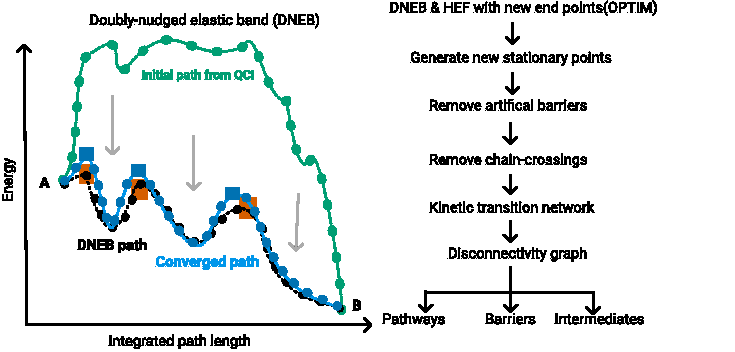
\includegraphics{Fig1.pdf}
    \caption{A cartoon depicting an OPTIM run. With local minima A and B as end-points, an initial path (series of images) is generated from quasi-continuous interpolation (QCI). The DNEB energy is then minimised until the gradient falls below a pre-defined threshold resulting in a DNEB optimised path. On this path, images that correspond to local maxima are identified as guessed transition states (GTS) depicted as red squares. These are used as starting guesses for transition state refinement using hybrid eigenvector-following resulting in a converged pathway comprising local minima and refined transition states. A successful OPTIM run results in a series of connected stationary points along the pathway. PATHSAMPLE then selects multiple pairs of end-points from a database of local minima that are connected with OPTIM in the manner described above. If a fully connected path has not been reached, new end-points for further DNEB searches with OPTIM are generated, and the procedure is repeated. The final database, after multiple connections have been found between many sets of end-points, contains local minima and the transition states that connect them in a kinetic transition network, which is then visualised as a disconnectivity graph with disconnectionDPS or Pyconnect\cite{Smeeton14a}. }
    \label{fig:flow}
\end{figure}

The next challenge is to sample the potential energy surface more extensively by ensuring we add more local minima and transition states to our database  to improve the representation of overall kinetics and thermodynamics. For this purpose, we use the PATHSAMPLE program \cite{PATHSAMPLE}. PATHSAMPLE offers multiple strategies for selection of pairs of minima (one minimum corresponding to the reactant A and another corresponding to a product B) for connection attempts. These include:
\begin{itemize}
    \item {Reactant-product (or AB) pairs can be selected for connection attempts based on the highest barrier on the path that makes the largest contribution to the rate constant  (DIJPAIRS\cite{Strodel07a}).}
    \item{To eliminate artificial frustration and increase the size of the database, a disconnectivity analysis can be performed and connections attempted between all minima and any of the minima in the product set based on the largest barriers in the product direction.  (UNTRAP\cite{Strodel07a})}
    \item{Unconnected pairs of reactants and products are automatically selected from the database to connect minima not already connected to the AB region (CONNECTUNC\cite{Roder18a})}
    \item{Find shorter pathways from already existing pathways between reactant and product states in the database (SHORTCUT and SHORTCUT BARRIER\cite{Carr05a,Strodel07a}). Typically, used for post-processing.}
    \item {The database of stationary points is regrouped by combining free energy minima where forward and backward free energy barriers are both less than a pre-defined energy value. Pairs of potential energy minima are then  chosen from groups based on the ratio of free energy barrier height to product divided by free energy difference from product. Local minima from these free energy groups are then chosen based upon an additional shortest distance criterion.((FREEPAIRS\cite{Carr08a})}
    \item{Finally, a list of pairs of minima to be connected can be manually provided as an external file (CONNECTPAIRS). }
\end{itemize}


Here, in order to perform a more exhaustive search to populate the potential energy landscape, we use the UNTRAP\cite{Strodel07a} keyword. Pairs of minima to be connected are automatically selected and DNEB runs between each pair are performed. All new distinct local minima and transition states found from each DNEB run are written to a database. PATHSAMPLE automatically initiates and tracks multiple independent OPTIM runs can be distributed over multiple processors. 

In the first PATHSAMPLE run, we add all the paths found from the  OPTIM runs carried out in the previous section. This step populates the database with the corresponding minima and transition states. We run PATHSAMPLE a second time to automatically select pairs of local minima for new connection attempts between pairs of minima from the populated database and build the database further. 

Four files \emph{min.data}, \emph{ts.data}, \emph{points.min} and \emph{points.ts} contain the database of stationary points. Minima and transition states are ranked in the order of appearance in the min.data and ts.data files, which contain information about the potential energy and properties needed to calculate the partition functions and rate constants such as normal mode frequencies and moments of inertia. The last two files contain Cartesian coordinates of each local minimum and transition state respectively stored in direct access format. 

The \emph{pathdata} file contains instructions for controlling the PATHSAMPLE run. A list of keywords for the \emph{pathdata} file can be found in Ref.\cite{PATHSAMPLE}. An example \emph{pathdata} file is provided in the SI. An \emph{odata.connect} file contains instructions for the OPTIM runs that are to be performed with PATHSAMPLE, analogous to the \emph{odata} file from the first section.

\begin{itemize}
    \item {Copy path.info files as \emph{path1,path2,..pathN} in a new folder. Use keyword ADDPATH path1, ADDPATH path2,..ADDPATH pathN in the \emph{pathdata} file to populate an initial database of minima and transition states\\  \tt{./PATHSAMPLE}}
    \item {Comment out the ADDPATH keywords and instead add the UNTRAP keyword\footnote{See \url{http://www-wales.ch.cam.ac.uk/PATHSAMPLE.2.1.doc/node5.html} for a for a list of keywords for the pathdata file} keyword to the \emph{pathdata} file with appropriate values. Ensure the odata.connect and SBM.INP files are in the working directory. \\ \tt{./PATHSAMPLE}}
\end{itemize}
% \footnote{For \emph{PATHSAMPLE} runs on parallel computing, the SLURM job scheduling system is recommended. Support for the Portable Batch System (PBS) is also provided but the SSH keyword in needs to be present in the \emph{pathdata} file.}

\subsubsection{Visualising and analysing the database}
The potential energy surface is partitioned into basins of attraction where each point on the landscape is mapped onto a local minimum by a steepest-descent path. A hierarchical clustering of local minima is performed based on the potential energy barriers separating them. Starting from the energy of the native state, regions on the landscape are clustered together if they are separated by a barrier below a pre-defined energy threshold. Clustering is repeated until a maximum energy threshold is reached. The resulting graph representation (a coarse-grained representation of the potential energy surface) is referred to as a disconnectivity graph. Local minima are represented as nodes on the graph. Edges are bidirectional comprising rate constants in both directions from reactant to product states. The connectivity of the graph defines the nature of the underlying potential energy surface. For a smooth funnel, it manifests in a ``palm-tree'' like shape with one pronounced branch leading to the bottom of the funnel (the native-state). Other populated basins (kinetic traps) connected to the native state, appear as sub-funnels with separate branches. Disconnectivity graphs retain both the energies of minima on the potential energy surface, and the potential energy barriers that separate them. An important advantage of this representation is that it captures  full-dimensionality of the energy landscape without having to rely on a projection to a pre-defined order. 

To plot a disconnectivity graph with \emph{disconnectionDPS}, we need  \emph{min.data} and \emph{ts.data} files generated from the \emph{PATHSAMPLE} runs. A \emph{dinfo} file provides input information such as the pre-defined energy threshold, size of the energy window, identifying minima on the landscape and plotting an order parameter by colour, among others. Example of a dinfo file is provided in Supplementary Information.

\begin{itemize}
\small
    \item {With \emph{min.data}, \emph{ts.data} and \emph{dinfo} files in folder : \tt{./disconnectionDPS}}
\end{itemize}

Software for plotting metric disconnectivity graphs with the data generated from PATHSAMPLE, called PYCONNECT, was developed by Smeeton and Johnston\cite{Smeeton14a}. Given that the landscape is described as a bidirectional graph, a k-shortest path algorithm\cite{Sharpe19a} can be used to find multiple distinct paths between any two local minima described as nodes with the KDISTINCTPATHS keyword \cite{PATHSAMPLE1} in the \emph{pathdata} file and run \emph{PATHSAMPLE}. 

\subsubsection{Knot classification}
Each local minimum found in the database is classified by knot type with the Kymoknot program\cite{Tubiana18a}. UCH-L1 is an open-chain protein while knots are strictly defined only in closed loops. The open-chain protein is closed by a minimally interfering chain closure scheme \cite{Tubiana18a} (See Figure \ref{fig:fig2}b). The knotted core is determined by the KMT reduction algorithm\cite{Koniaris91a}. To identify the knot type of the closed loop, the Alexander polynomial is computed. 

\section{Results}
\subsection{Energy landscape of UCH-L1- A protein with a knotted topology}

\begin{figure}
    \centering
    \includegraphics[width=0.8\textwidth]{Fig2.pdf}
    \caption{ (a) A depiction of an ideal 5$_2$ or Gordian knot formed with a closed loop coloured in the N- to C-direction from blue to red. (b) Sketch of backbone and loop-closure between the N- and C-termini of UCH-L1 resulting in the 5$_2$ knot classification and (c) Secondary structure of the UCH-L1 protein with the terminal residues and secondary structure showing 9 $\alpha$-helices and 6 $\beta$-sheets.\label{fig:fig2}}
\end{figure}

\begin{figure}
    \centering
    \includegraphics[width=0.8\textwidth]{Fig3.pdf}
    \caption{Disconnectivity graph for UCH-L1 comprising 11126 minima and 15582 transition states. Gordian (orange nodes), figure-of-eight (blue nodes) and trefoil (green nodes) knots were found on the landscape. Three clear sub-basins, D1, D2 and D3 emerge. D2 corresponds to a jammed trefoil knot while D1, and D3 sub-basins remain unknotted.\label{fig:fig3}}
\end{figure}

The energy landscape for UCH-L1 appears largely well-funnelled with three major sub-basins. The funneled nature of the energy landscape supports the experimental unfolding and re-folding observed in denaturant.  In the disconnectivity graph (Figure \ref{fig:fig3}), 9.6\% of the minima are classified as trefoil knots, 0.3\%  as figure-of-eight knots and the rest as unknots. Gordian knots were observed up to an energy of 55$\varepsilon$ above the native state. 

One sub-basin of unknotted structures, D1 (barrier of 10$\varepsilon$), was found within this energy range. The sub-basin D2 (barrier of 30$\varepsilon$)  contained only trefoil knots indicating the presence of a topological trap in a jammed trefoil-knotted state, while sub-basin D3 contained only unknotted structures. There are many trefoil knotted structures in the database of local minima that do not belong to the basin D2. All three kinetic traps, D1, D2 and D3 remain stable on addition of side-chains\cite{Wang08a} during a low-temperature molecular dynamics simulation of 100ns with an all-atom AMBER ff14SB potential with and implicit solvent Born model (details in SI).  
\subsection{Pathways to the	Gordian knot}
\begin{figure}
    \centering
    \includegraphics[width=\textwidth]{Fig4.pdf}
    \caption{Folding pathways from 1000 highest energy local minima found on the landscape classified by topology of structures found along the folding pathway. Knot-type for every stationary point on each pathway was found and classified as unknot (Un), trefoil(Tr), figure-of-eight(F8) or Gordian(Gdn) knot. x-axis is the number of stationary points visited, y-axis is relative energy ($\varepsilon$) and the z-axis is the knot type of each stationary point. Topologically distinct pathways are sketched by knot type next to each plot. If the tail on the N-terminus exits first, we always see the formation of a trefoil knot followed by an unknot. If the longer C-terminus exits first, two possible pathways emerge, in one case direct conversion to an unknot occurs and in the second, conversion to an unknot is followed by a figure-of-eight knot and then back to an unknot. Schematic figures of knots were plotted with Knotplot\cite{knotplot}.}
    \label{fig:fig4}
\end{figure}
Folding pathways obtained from 1000 highest energy local minima found on the disconnectivity graph leading to the native Gordian knotted state are depicted in Figure \ref{fig:fig3}, classified by the knot types identified along the pathway. (Un)knotting from the N-terminus, which comprises a smaller tail of five residues, is the most favoured mechanism. The tail is surrounded by a large flexible loop (residues 146-159 connecting $\alpha$7 and $\beta$3). The smaller tail on the N-terminus exits this loop resulting in a structure classified as an unknot. The $\alpha$7-$\alpha$8-$\beta$3 motif is quite flexible and opens up first resulting in unknotting (Figure \ref{fig:fig4}a). It is also possible for the C-terminus to untie while the N-terminus remains inside the loop. This mechanism results in a structure that is classified as a trefoil knot(Figure \ref{fig:fig4}b). The tail at the C-terminus has 10 residues. 

In most cases, this tail exits the loop formed by $\alpha$1-$\beta$1 motif resulting in a trefoil knotted intermediate. Interestingly, we also found a few structures classified as figure-of-eight knots on the folding pathway. This motif occurs when both the N- and C-termini untie and then the C-terminus enters the large loop previously occupied by the N-terminus (Figure \ref{fig:fig4}c). In this pathway, the protein unknots, forms a figure-of-eight knot, unknots again and then forms a Gordian knot.  Pathways similar to the ones identified were also seen from molecular dynamics simulations with an identical coarse-grained SBM potential\cite{Zhao18a} at the folding temperature (the temperature where folded zand unfolded states are equally populated in the ensemble). 

\section{Conclusion}
With the example of a complex and functionally important protein, UCH-L1, we show how the discrete path sampling methodology can be employed in combination with Structure-Based Models to construct a detailed energy landscape from which parallel folding pathways can be extracted along with kinetic traps and potential energy barriers for important conformational transitions. We reproduce known topologically distinct folding pathways found for this protein found from molecular dynamics simulations with an identical potential. In addition, we identify topological traps and quantify the topological barriers that separate them from the native 5$_2$ knotted state. 
%\bibliographystyle{els}
\bibliography{sample.bib}

\end{document}
